\chapter{Wykład 9. Zarządzanie czasem w projekcie informatycznym}

\section{SPP uwzglęniający plan kont kosztowych projektu}
% strona 34

\begin{figure}[hbt]
\centering
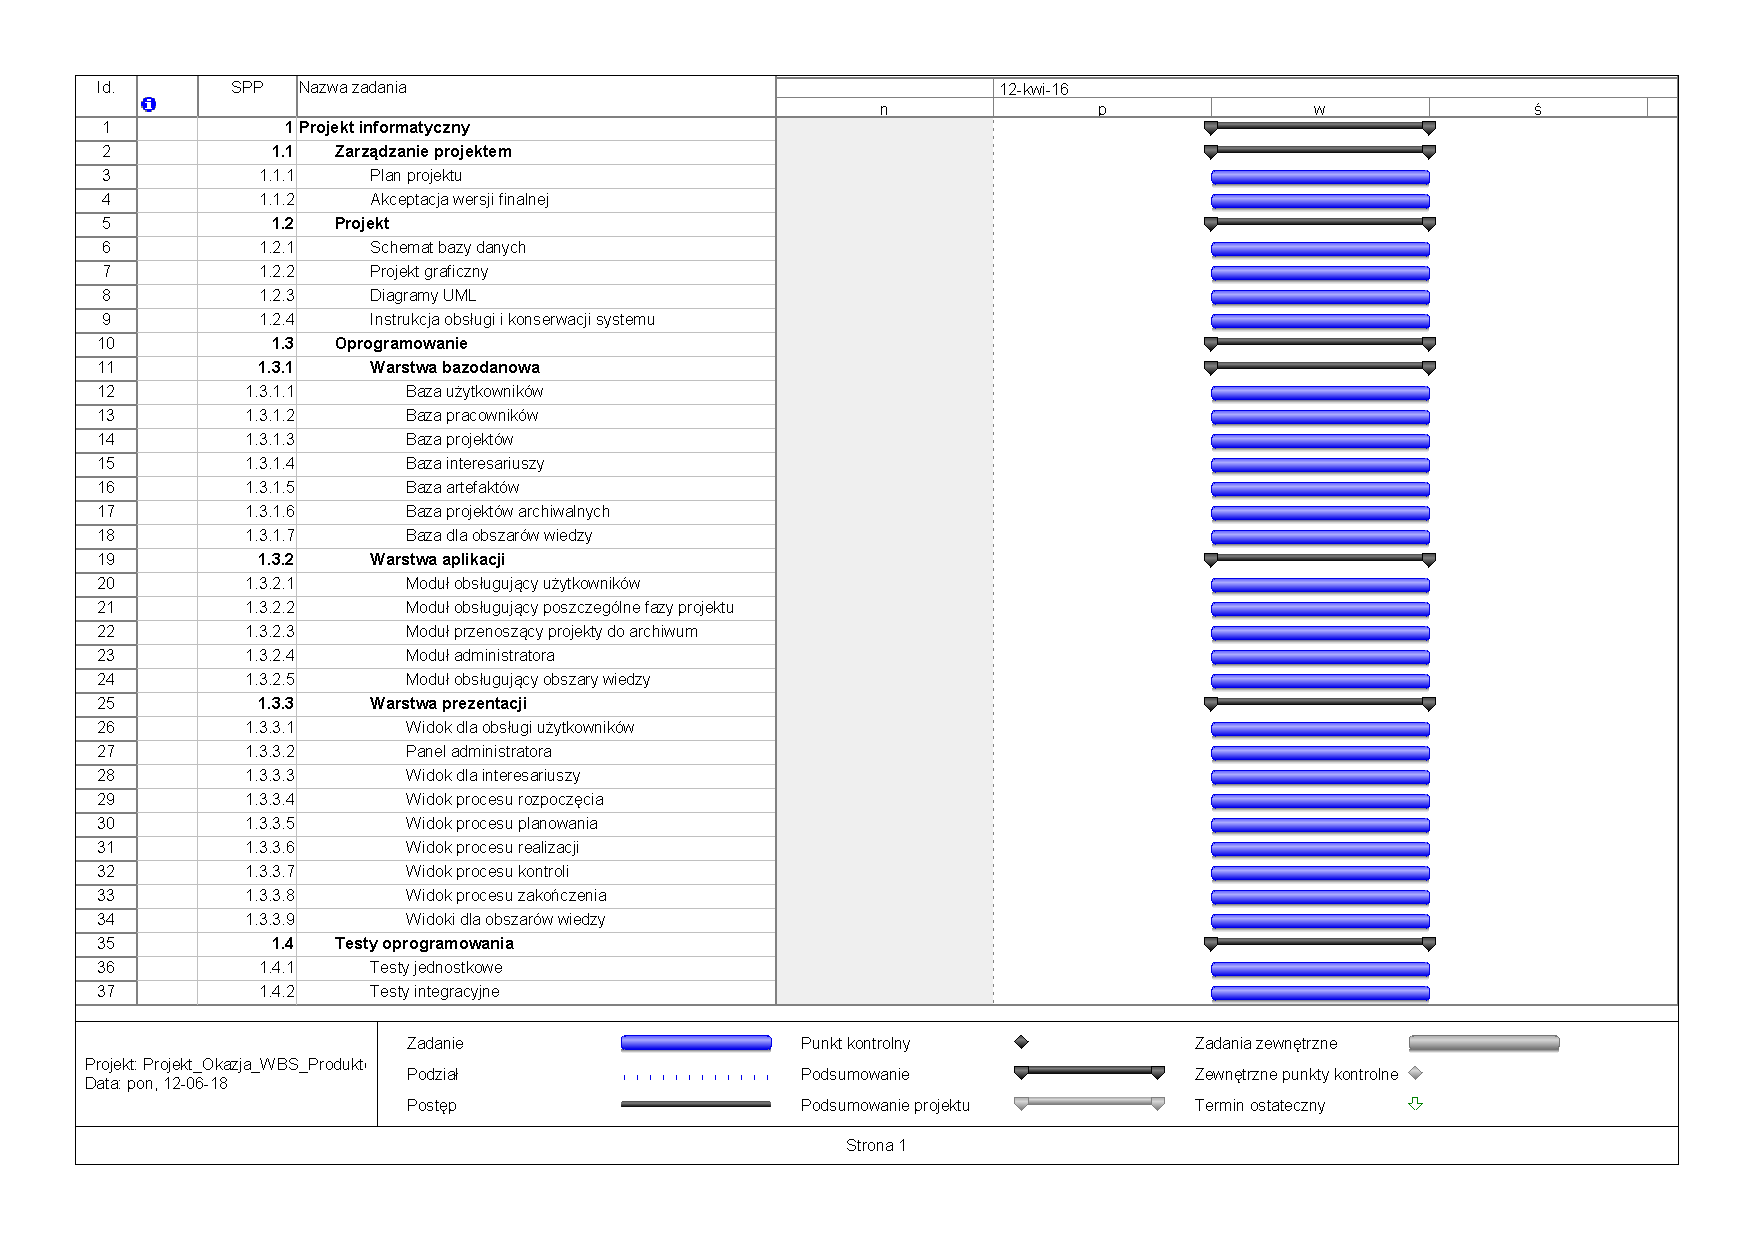
\includegraphics[width=1.1\textwidth]{diagramSPP.pdf}
\caption{Diagram SPP}
\label{fig:diagramSPP}
\end{figure}

% ===========================================================================

\section{Harmonogram w MS Project}
% strona 35

\begin{figure}[hbt]
\centering
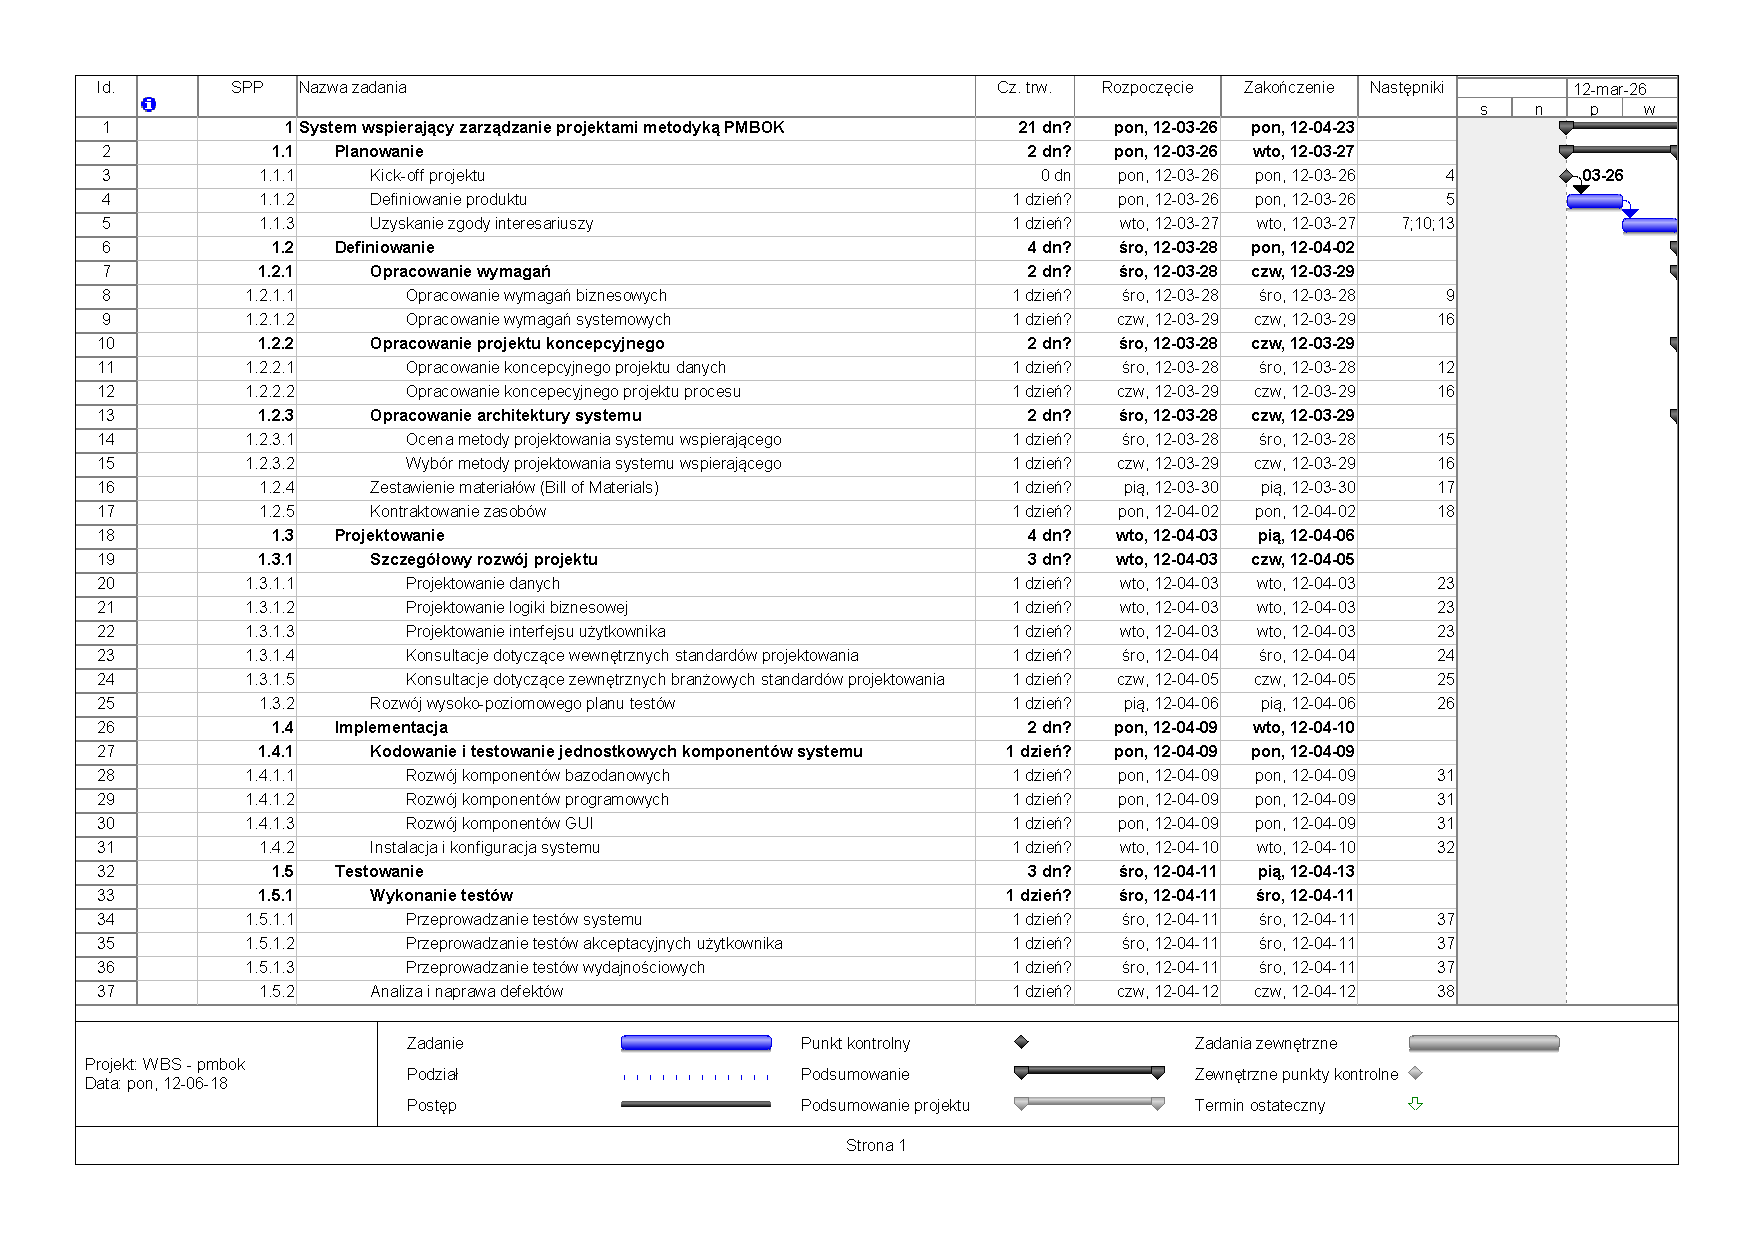
\includegraphics[width=1.1\textwidth]{harmonogramWBS.pdf}
\caption{Harmonogram}
\label{fig:harmonogramWBS}
\end{figure}

% ===========================================================================

\section{Struktura RBS projektu}
% strona 45

\begin{figure}[h]
\begin{center}
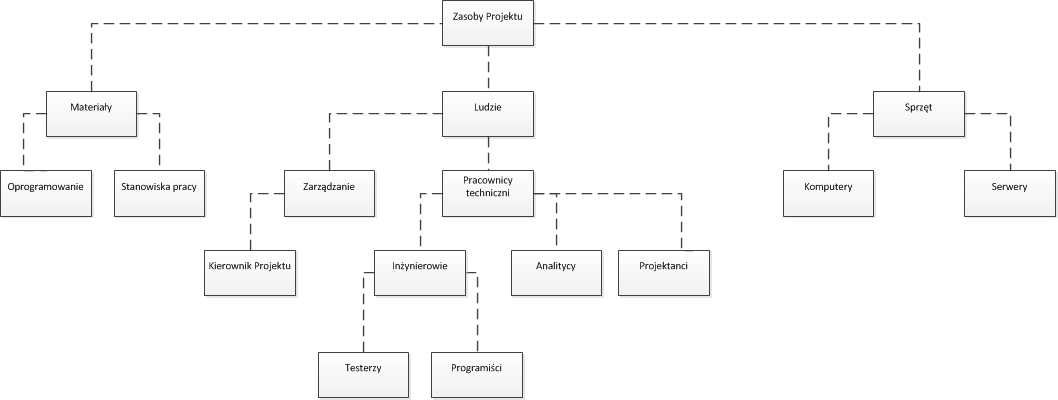
\includegraphics[scale=0.6]{RBS.png}
\caption[RBS]{RBS}
\label{rysunekProces}
\end{center}
\end{figure}

% ===========================================================================

\section{Harmonogram z uwzględnieniem zasobów}
% strona 59

Ten wirtualny warsztat jest beznadziejny.


